\chapter{Biomoléculas: aminoácidos, açúcares, lipídios e nucleotídeos}\label{ch:b2:biomolecules}

Um adoçante comum, muito mais doce que o açúcar, é formado por dois aminoácidos unidos por uma única
ligação amida, um deles na forma de éster metílico: o ácido aspártico e a fenilalanina, ambos com a
configuração que as células vivas usam. As moléculas da vida são construídas a partir de algumas
famílias de pequenas unidades, aminoácidos, açúcares, \omterm{def:b2:biomolecules:lipid}{ácidos graxos} e \omterm{def:b2:biomolecules:nucleotide}{nucleotídeos}, unidas pelas reações
dos capítulos anteriores: amidas, acetais, ésteres. Este capítulo as lê como um químico orgânico:
grupos funcionais, estereoquímica, comportamento ácido--base, e as reações que as unem e as cortam.
% ledger: use:aspartame

\begin{recall}
O volume do 1.º ano: regras CIP, projeções de Fischer, quiralidade, hemiacetais e acetais, $\mathrm pK_a$
e diagramas de distribuição, moléculas anfifílicas, lei de Biot. \Cref{ch:b2:acyl-substitution}: amidas,
ésteres, \omterm{def:b2:acyl-substitution:saponification}{saponificação}, ácidos ativados. \Cref{ch:b2:amines}: as aminas como bases.
\Cref{ch:b2:retrosynthesis}: os grupos protetores em uma via.
\end{recall}

\section{Os aminoácidos}

\begin{definition}[Aminoácidos]\label{def:b2:biomolecules:amino-acid}
Um \emph{$\alpha$-aminoácido}\index{alfa-aminoacido@$\alpha$-aminoácido} \ce{H2N-CHR-COOH} leva um grupo
amino e um grupo ácido carboxílico no mesmo carbono; \ce{R} é sua \emph{cadeia
lateral}\index{cadeia lateral}. Em água perto do pH neutro, ele existe como \emph{zwitteríon}\index{zwitterion@zwitteríon},
\ce{H3N+-CHR-COO-}, que leva uma carga positiva e uma negativa. O \emph{ponto
isoelétrico}\index{ponto isoeletrico@ponto isoelétrico} pI é o pH no qual sua carga líquida média é nula.
\end{definition}

Vinte aminoácidos constroem as proteínas dos seres vivos. Todos, exceto a glicina (\ce{R = H}), são
quirais, e os naturais têm a configuração L (\cref{def:b2:biomolecules:d-l}). Suas \omterm{def:b2:biomolecules:amino-acid}{cadeias laterais} os
repartem em famílias: apolares (alanina, \ce{R = CH3}; fenilalanina, \ce{R = CH2C6H5}), polares, ácidos
(ácidos aspártico e glutâmico, com um segundo grupo carboxílico) e básicos (lisina, com um segundo grupo
amino; histidina, com um anel imidazol).

\begin{proposition}[Ponto isoelétrico]\label{prop:b2:biomolecules:pi}
Para um aminoácido cuja \omterm{def:b2:biomolecules:amino-acid}{cadeia lateral} não é nem ácida nem básica, $\mathrm{pI} = (\mathrm pK_{a1} +
\mathrm pK_{a2})/2$, onde $\mathrm pK_{a1}$ pertence ao grupo carboxílico e $\mathrm pK_{a2}$ ao
grupo amônio. Para uma \omterm{def:b2:biomolecules:amino-acid}{cadeia lateral} ácida ou básica, o pI é a média dos dois $\mathrm pK_a$ que
enquadram a forma neutra.
\end{proposition}

\begin{proof}
Escrevamos \ce{H2A+} para o cátion, \ce{HA} para o \omterm{def:b2:biomolecules:amino-acid}{zwitteríon} e \ce{A-} para o ânion. A carga líquida é
nula quando $[\ce{H2A+}] = [\ce{A-}]$. De $K_{a1} = [\ce{HA}]h/[\ce{H2A+}]$ e $K_{a2} =
[\ce{A-}]h/[\ce{HA}]$, com $h = [\ce{H3O+}]$, a razão $[\ce{H2A+}]/[\ce{A-}] = h^2/(K_{a1}K_{a2})$
vale 1 para $h^2 = K_{a1}K_{a2}$, isto é, $\mathrm{pH} = (\mathrm pK_{a1} + \mathrm pK_{a2})/2$. Com um
terceiro grupo ionizável, o mesmo argumento se aplica aos dois equilíbrios situados de cada lado da
forma neutra, estando o terceiro grupo então inteiramente em um estado.
\end{proof}

Para a glicina, $\mathrm pK_{a1} = 2.35$ e $\mathrm pK_{a2} = 9.78$: pI $\approx 6.1$. O ácido aspártico
(2.0, 3.9, 9.9) tem pI $\approx 3.0$; a lisina (2.2, 9.1, 10.7) tem pI $\approx 9.9$.
% ledger: pka:glycine1, pka:glycine2, pka:asp1, pka:asp2, pka:asp3, pka:lys1, pka:lys2, pka:lys3

\begin{omfigure}
\begin{tikzpicture}
\begin{axis}[width=0.47\linewidth, height=5cm, xmin=0, xmax=14, ymin=-2.2, ymax=2.2,
  xlabel={pH}, ylabel={carga líquida}, label style={font=\small}, tick label style={font=\scriptsize},
  xtick={0,2,4,6,8,10,12,14}, ytick={-2,-1,0,1,2}, grid=major, grid style={black!12},
  legend style={font=\scriptsize, at={(0.5,1.03)}, anchor=south}, legend columns=3]
\addplot[omDef, thick] table[x=pH, y=gly] {figdata/out/bachelor-2-amino-acid-charge-a.dat};
\addplot[omThm, thick] table[x=pH, y=asp] {figdata/out/bachelor-2-amino-acid-charge-a.dat};
\addplot[omMeth, thick] table[x=pH, y=lys] {figdata/out/bachelor-2-amino-acid-charge-a.dat};
\legend{glicina, ácido aspártico, lisina}
\end{axis}
\end{tikzpicture}\hfill
\begin{tikzpicture}
\begin{axis}[width=0.47\linewidth, height=5cm, xmin=0, xmax=14, ymin=0, ymax=1.05,
  xlabel={pH}, ylabel={fração}, label style={font=\small}, tick label style={font=\scriptsize},
  xtick={0,2,4,6,8,10,12,14},
  legend style={font=\scriptsize, at={(0.5,1.03)}, anchor=south}, legend columns=3]
\addplot[omThm, thick] table[x=pH, y=cation] {figdata/out/bachelor-2-amino-acid-charge-b.dat};
\addplot[omDef, thick] table[x=pH, y=zwitterion] {figdata/out/bachelor-2-amino-acid-charge-b.dat};
\addplot[omMeth, thick] table[x=pH, y=anion] {figdata/out/bachelor-2-amino-acid-charge-b.dat};
\legend{cátion, zwitteríon, ânion}
\end{axis}
\end{tikzpicture}

{\small À esquerda: carga líquida de três aminoácidos em função do pH, a partir de seus $\mathrm pK_a$ a
\qty{25}{\degreeCelsius}; cada curva corta o zero no pI. À direita: as três formas da glicina,
\ce{H3N+CH2COOH}, \ce{H3N+CH2COO-} e \ce{H2NCH2COO-}; o \omterm{def:b2:biomolecules:amino-acid}{zwitteríon} predomina de cerca de pH 3 a
pH 9.}
% figdata: bachelor-2/amino-acid-charge.py parts a, b
\end{omfigure}

\begin{method}[Carga líquida a um pH dado]\label{met:b2:biomolecules:charge}
\begin{enumerate}
  \item Liste todos os grupos ionizáveis com seu $\mathrm pK_a$: o \ce{NH3+} e o \ce{COOH} terminais, e as
        \omterm{def:b2:biomolecules:amino-acid}{cadeias laterais} ionizáveis.
  \item Para cada grupo, compare o pH e o $\mathrm pK_a$: um grupo está sobretudo protonado abaixo de
        seu $\mathrm pK_a$, sobretudo desprotonado acima (por mais de 1 unidade: mais de 90~\%).
  \item Some as cargas: \ce{NH3+} $+1$, \ce{NH2} 0, \ce{COOH} 0, \ce{COO-} $-1$ (imidazólio $+1$).
  \item Perto de um $\mathrm pK_a$, conte esse grupo como meio carregado; para um valor exato, use as
        frações $1/(1 + 10^{\mathrm pK_a - \mathrm{pH}})$.
\end{enumerate}
\end{method}

\section{Os peptídeos}

\begin{definition}[Peptídeos]\label{def:b2:biomolecules:peptide}
A ligação amida formada entre o grupo carboxílico de um aminoácido e o grupo amino de outro é uma
\emph{ligação peptídica}\index{ligacao peptidica@ligação peptídica}; uma cadeia de aminoácidos unidos por ligações peptídicas é
um \emph{peptídeo}\index{peptideo@peptídeo} (uma proteína quando é longa), escrito a partir de sua extremidade amino
livre (N-terminal) até sua extremidade carboxílica livre (C-terminal). Um \emph{acoplamento
peptídico}\index{acoplamento peptidico@acoplamento peptídico} forma uma ligação peptídica no laboratório com um
\emph{agente de acoplamento}\index{agente de acoplamento}, um reagente que converte o grupo carboxílico em um
derivado ativado em condições brandas (uma carbodi-imida, por exemplo).
\end{definition}

\begin{omfigure}
\setchemfig{atom sep=1.9em}
\schemestart
\chemfig{R-C(=[2]O)-N(-[6]H)-R'}
\arrow{<->}
\chemfig{R-C(-[2]\chemabove{O}{\scriptstyle -})=\chemabove{N}{\scriptstyle +}(-[6]H)-R'}
\schemestop
\par\vspace{6pt}

{\small As duas estruturas de ressonância da \omterm{def:b2:biomolecules:peptide}{ligação peptídica}. O par não ligante do nitrogênio é
compartilhado com a carbonila: a ligação \ce{C-N} tem um caráter parcial de ligação dupla, e os seis
átomos C, C, O, N, H, C ficam em um mesmo plano.}
\end{omfigure}

\begin{proposition}[Uma ligação plana]\label{prop:b2:biomolecules:planar}
A \omterm{def:b2:biomolecules:peptide}{ligação peptídica} é plana, a rotação em torno da ligação \ce{C-N} é restrita, e o nitrogênio da amida
não é nem básico nem nucleofílico.
\end{proposition}

\begin{proof}[Raciocínio]
A segunda estrutura de ressonância dá à ligação \ce{C-N} uma parte de caráter de ligação dupla: girá-la
romperia a sobreposição do par não ligante do nitrogênio com o sistema $\pi$ \ce{C=O}, o que custa
energia, de modo que os átomos em torno dela ficam em um mesmo plano, sendo o arranjo trans (os dois
carbonos da cadeia de lados opostos da ligação \ce{C-N}) o habitual. O par não ligante engajado na
ressonância não está disponível para um próton ou um eletrófilo, como em toda amida
(\cref{ch:b2:acyl-substitution}). As proteínas se dobram em torno de cadeias desses planos rígidos.
\end{proof}

\begin{proposition}[Por que proteger e ativar]\label{prop:b2:biomolecules:coupling}
Preparar um dipeptídeo determinado a partir de dois aminoácidos exige ao mesmo tempo a proteção dos
grupos que não devem reagir e a ativação do grupo carboxílico que deve reagir.
\end{proposition}

\begin{proof}[Raciocínio]
Um ácido carboxílico e uma amina misturados à temperatura ambiente dão um sal, não uma amida; aquecer
para expulsar a água também racemizaria os aminoácidos. É preciso portanto uma ativação (um \omterm{def:b2:acyl-substitution:derivative}{cloreto de
acila}, um anidrido, ou um \omterm{def:b2:biomolecules:peptide}{agente de acoplamento}). Mas cada aminoácido tem os dois grupos: ativar uma
mistura de glicina e alanina daria Gly--Ala, Ala--Gly, Gly--Gly, Ala--Ala e cadeias mais longas. Bloquear
a amina do primeiro e o ácido do segundo deixa uma única ligação possível.
\end{proof}

\begin{method}[Síntese de um dipeptídeo]\label{met:b2:biomolecules:peptide}
\begin{enumerate}
  \item Proteja o grupo amino do aminoácido N-terminal (como carbamato, por exemplo um grupo
        \textit{terc}-butoxicarbonila).
  \item Proteja o grupo carboxílico do aminoácido C-terminal (como éster metílico ou benzílico), e toda
        \omterm{def:b2:biomolecules:amino-acid}{cadeia lateral} reativa.
  \item Ative o grupo carboxílico livre com um \omterm{def:b2:biomolecules:peptide}{agente de acoplamento} e acrescente o parceiro protegido:
        forma-se uma \omterm{def:b2:biomolecules:peptide}{ligação peptídica}.
  \item Remova os grupos protetores, de preferência um conjunto ortogonal
        (\cref{def:b2:retrosynthesis:orthogonal}); para continuar, remova apenas a proteção da amina e repita.
\end{enumerate}
\end{method}

Repetir o ciclo muitas vezes em solução exigiria uma purificação a cada etapa. Na síntese em fase
sólida, a cadeia em crescimento está presa por seu C-terminal a uma esfera de \omterm{def:b2:polymer-synthesis:polymer}{polímero}; os reagentes em
excesso e os subprodutos são eliminados por lavagem após cada acoplamento, e o \omterm{def:b2:biomolecules:peptide}{peptídeo} acabado é
separado do suporte no final.

\begin{omfigure}
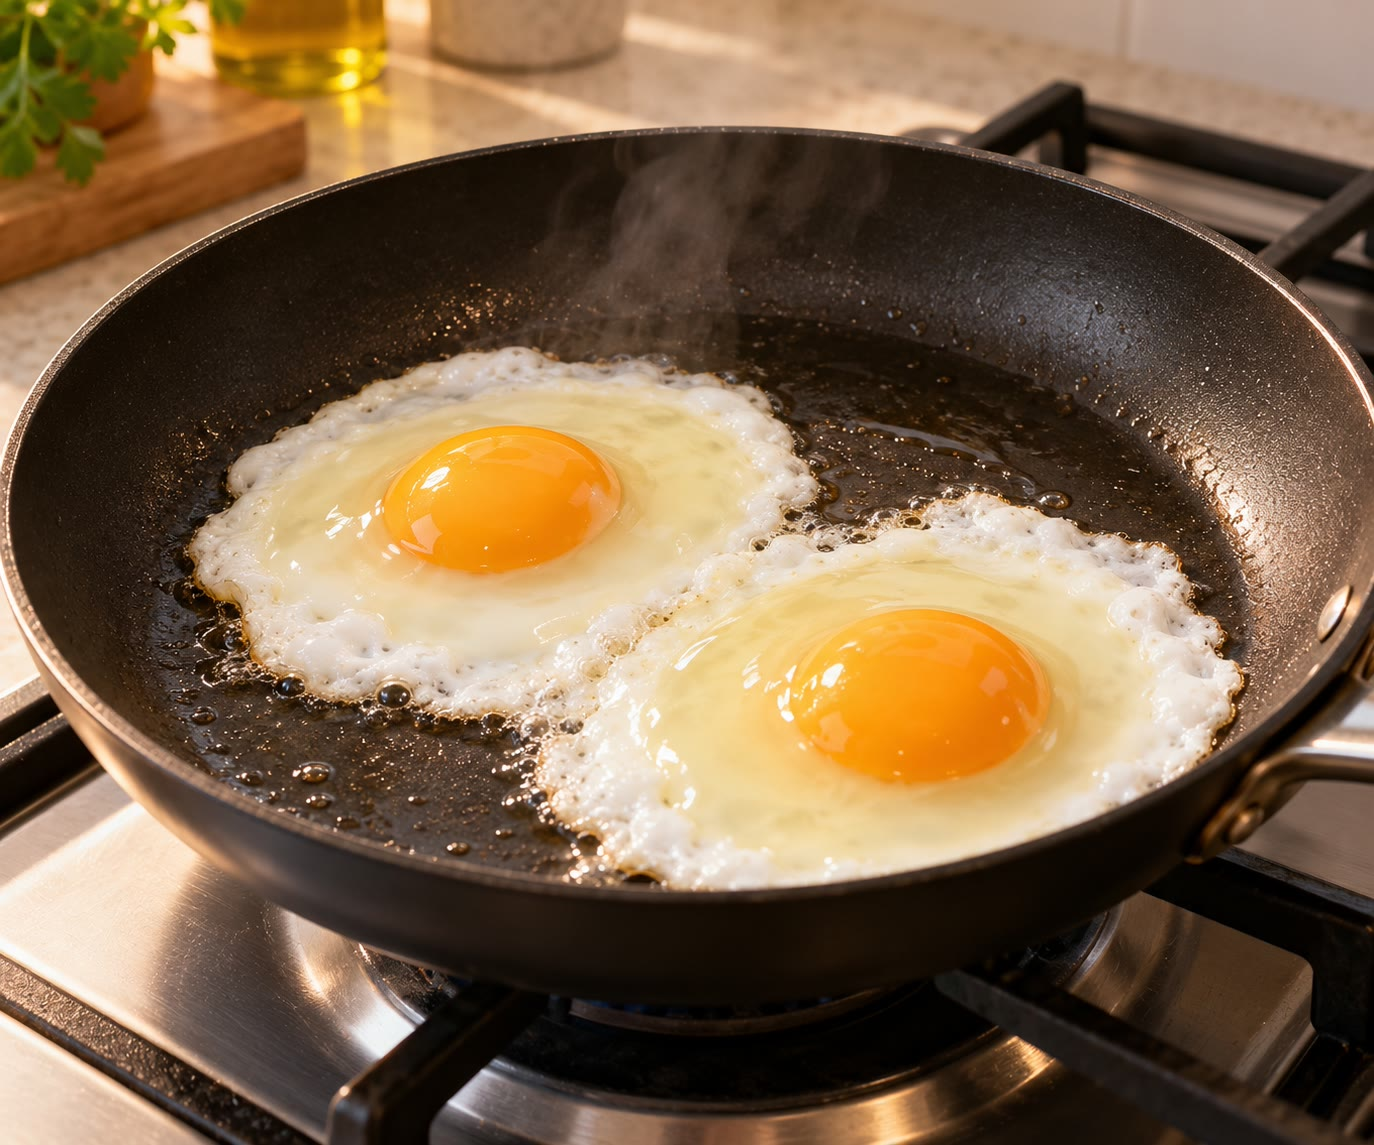
\includegraphics[width=0.5\linewidth]{images/book3/ai/b2-30-eggs.jpg}

{\small Ovos fritando. As proteínas da clara se desdobram com o aquecimento e se ligam umas às outras:
o líquido translúcido se transforma em um sólido branco opaco. Nenhuma \omterm{def:b2:biomolecules:peptide}{ligação peptídica} se rompe; a
mudança está na maneira como as cadeias estão dobradas (ilustração).}
\end{omfigure}

\section{Os glicídios}

\begin{definition}[D e L]\label{def:b2:biomolecules:d-l}
Um açúcar ou um aminoácido é desenhado em projeção de Fischer com seu carbono mais oxidado no alto. Ele
é D se o \ce{OH} do estereocentro mais afastado do alto (ou, para um $\alpha$-aminoácido, o
\ce{NH2} do carbono $\alpha$) aponta para a direita, e L se aponta para a esquerda. Os descritores
comparam as configurações com a do gliceraldeído; não são os descritores CIP.
\end{definition}

\begin{definition}[Monossacarídeos]\label{def:b2:biomolecules:sugar}
Um \emph{monossacarídeo}\index{monossacarideo@monossacarídeo} é um poli-hidroxialdeído ou uma poli-hidroxicetona, em geral
\ce{C_nH_{2n}O_n} com $n$ de 3 a 7, que não pode ser hidrolisado em açúcares menores. Uma
\emph{aldose}\index{aldose} tem um grupo aldeído em C1, uma \emph{cetose}\index{cetose} um grupo cetona,
em geral em C2. A glicose é uma aldo-hexose, a frutose uma ceto-hexose.
\end{definition}

Em água, uma aldo-hexose é quase inteiramente cíclica: o \ce{OH} de C5 se adiciona ao aldeído, formando
um anel hemiacetal de seis membros (uma piranose). A ciclização cria um novo estereocentro em C1.

\begin{definition}[Anômeros]\label{def:b2:biomolecules:anomer}
Em uma \emph{projeção de Haworth}\index{projecao de Haworth@projeção de Haworth} o anel de um açúcar cíclico é desenhado plano,
perpendicular à página, com seu oxigênio atrás à direita e seus substituintes acima ou abaixo do
anel. O carbono hemiacetálico (C1 de uma \omterm{def:b2:biomolecules:sugar}{aldose}) é o \emph{carbono anomérico}\index{carbono anomerico@carbono anomérico}; as
duas configurações que ele pode adotar dão dois diastereoisômeros, os \emph{anômeros}\index{anomeros@anômeros}: para
um açúcar D, o $\alpha$ tem o \ce{OH} anomérico abaixo do anel (oposto ao \ce{CH2OH}), o $\beta$ acima.
Em água, os anômeros se interconvertem passando pela cadeia aberta, e a rotação óptica de um anômero
recém-dissolvido deriva para um valor de equilíbrio: a \emph{mutarrotação}\index{mutarrotacao@mutarrotação}.
\end{definition}

\begin{omfigure}
\setchemfig{atom sep=1.7em}
\begin{minipage}[c]{0.24\linewidth}\centering
\chemfig{CHO-[6]C(-[4]H)(-[0]OH)-[6]C(-[4,,,2]HO)(-[0]H)-[6]C(-[4]H)(-[0]OH)-[6]C(-[4]H)(-[0]OH)-[6]CH_2OH}
\end{minipage}%
\begin{minipage}[c]{0.37\linewidth}\centering
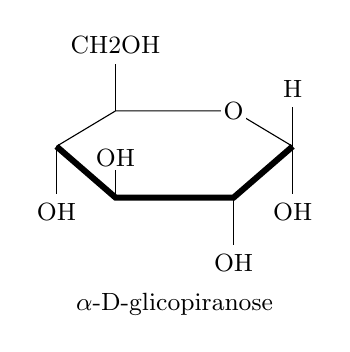
\begin{tikzpicture}[x=1cm, y=1cm, font=\small]
\coordinate (C4) at (-1.5,0); \coordinate (C3) at (-0.75,-0.65); \coordinate (C2) at (0.75,-0.65);
\coordinate (C1) at (1.5,0); \coordinate (O) at (0.75,0.45); \coordinate (C5) at (-0.75,0.45);
\draw (C5) -- (O) -- (C1); \draw (C4) -- (C5);
\draw[line width=2.2pt] (C4) -- (C3) -- (C2) -- (C1);
\node[fill=white, inner sep=1pt] at (O) {O};
\draw (C5) -- ++(0,0.6) node[above] {\ce{CH2OH}};
\draw (C1) -- ++(0,-0.6) node[below] {OH}; \draw (C1) -- ++(0,0.5) node[above] {H};
\draw (C2) -- ++(0,-0.6) node[below] {OH}; \draw (C3) -- ++(0,0.35) node[above, inner sep=1pt] {OH};
\draw (C4) -- ++(0,-0.6) node[below] {OH};
\node at (0,-2.0) {$\alpha$-D-glicopiranose};
\end{tikzpicture}
\end{minipage}%
\begin{minipage}[c]{0.37\linewidth}\centering
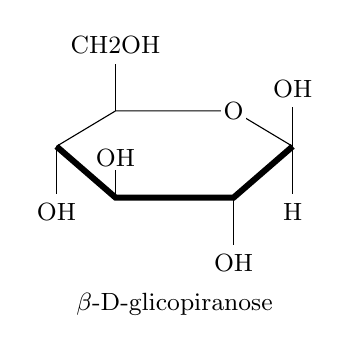
\begin{tikzpicture}[x=1cm, y=1cm, font=\small]
\coordinate (C4) at (-1.5,0); \coordinate (C3) at (-0.75,-0.65); \coordinate (C2) at (0.75,-0.65);
\coordinate (C1) at (1.5,0); \coordinate (O) at (0.75,0.45); \coordinate (C5) at (-0.75,0.45);
\draw (C5) -- (O) -- (C1); \draw (C4) -- (C5);
\draw[line width=2.2pt] (C4) -- (C3) -- (C2) -- (C1);
\node[fill=white, inner sep=1pt] at (O) {O};
\draw (C5) -- ++(0,0.6) node[above] {\ce{CH2OH}};
\draw (C1) -- ++(0,0.5) node[above] {OH}; \draw (C1) -- ++(0,-0.6) node[below] {H};
\draw (C2) -- ++(0,-0.6) node[below] {OH}; \draw (C3) -- ++(0,0.35) node[above, inner sep=1pt] {OH};
\draw (C4) -- ++(0,-0.6) node[below] {OH};
\node at (0,-2.0) {$\beta$-D-glicopiranose};
\end{tikzpicture}
\end{minipage}
\par\vspace{6pt}

{\small A D-glicose. À esquerda: a cadeia aberta em projeção de Fischer, \ce{OH} de C5 à direita (D). No
meio e à direita: os dois \omterm{def:b2:biomolecules:anomer}{anômeros} piranose em \omterm{def:b2:biomolecules:anomer}{projeção de Haworth}; os grupos à direita na projeção de
Fischer apontam para baixo, os da esquerda para cima, e C5 leva o \ce{CH2OH} para cima. Os \omterm{def:b2:biomolecules:anomer}{anômeros}
diferem apenas em C1. Os hidrogênios de C2 a C5 foram omitidos.}
\end{omfigure}

\begin{method}[De Fischer a Haworth (D-aldopiranose)]\label{met:b2:biomolecules:haworth}
\begin{enumerate}
  \item Desenhe o anel com O atrás à direita, C1 à direita, depois C2, C3, C4 no sentido horário pela
        frente e pela esquerda, C5 atrás à esquerda.
  \item Os grupos à direita na projeção de Fischer vão para baixo, os da esquerda para cima.
  \item Em C5 (série D), o \ce{CH2OH} vai para cima.
  \item Em C1, o \ce{OH} vai para baixo para $\alpha$, para cima para $\beta$.
\end{enumerate}
\end{method}

\begin{proposition}[Equilíbrio de mutarrotação]\label{prop:b2:biomolecules:mutarotation}
Se as rotações específicas dos \omterm{def:b2:biomolecules:anomer}{anômeros} puros são $[\alpha]_\alpha$ e $[\alpha]_\beta$ e a da mistura
em equilíbrio é $[\alpha]_{\mathrm{eq}}$, a fração molar do anômero $\alpha$ no
equilíbrio é
\begin{equation*}
x_\alpha = \frac{[\alpha]_{\mathrm{eq}} - [\alpha]_\beta}{[\alpha]_\alpha - [\alpha]_\beta}.
\end{equation*}
\end{proposition}

\begin{proof}
A cadeia aberta é uma fração ínfima da mistura e é desprezada. As rotações dos dois \omterm{def:b2:biomolecules:anomer}{anômeros} se somam
proporcionalmente a suas concentrações (lei de Biot, volume do 1.º ano); como eles têm a mesma massa
molar, $[\alpha]_{\mathrm{eq}} = x_\alpha[\alpha]_\alpha + (1 - x_\alpha)[\alpha]_\beta$, que se
resolve em $x_\alpha$.
\end{proof}

A D-glicose em equilíbrio em água tem $[\alpha] = +52.7$ (em \unit{\degree\,dm^{-1}\,g^{-1}\,mL}).
Com rotações dos \omterm{def:b2:biomolecules:anomer}{anômeros} de $+112$ e $+18.7$ (dados do exercício), $x_\alpha = (52.7 - 18.7)/(112 - 18.7)
\approx 0.36$: cerca de 36~\% de $\alpha$ e 64~\% de $\beta$. O anômero $\beta$, com todos os seus
substituintes equatoriais na cadeira, é o mais estável.
% ledger: rot:glucose-eq

\begin{definition}[Glicosídeos]\label{def:b2:biomolecules:glycoside}
Um \emph{glicosídeo}\index{glicosideo@glicosídeo} é o acetal formado quando o \ce{OH} anomérico de um açúcar é
substituído por um grupo \ce{OR} vindo de um álcool, muitas vezes outro açúcar; a ligação do \omterm{def:b2:biomolecules:anomer}{carbono
anomérico} a esse oxigênio é a \emph{ligação glicosídica}\index{ligacao glicosidica@ligação glicosídica}. Um \emph{açúcar redutor}\index{acucar redutor@açúcar redutor}
é um açúcar que reduz oxidantes brandos como o licor de Fehling ou o reagente de Tollens.
\end{definition}

\begin{proposition}[Redutor ou não]\label{prop:b2:biomolecules:reducing}
Um açúcar com um grupo hemiacetal (ou hemicetal) livre é redutor; um \omterm{def:b2:biomolecules:glycoside}{glicosídeo} cujos \omterm{def:b2:biomolecules:anomer}{carbonos
anoméricos} estão todos engajados em \omterm{def:b2:biomolecules:glycoside}{ligações glicosídicas} não é.
\end{proposition}

\begin{proof}[Raciocínio]
Um hemiacetal está em equilíbrio com a cadeia aberta, cujo grupo aldeído é oxidado pelo reagente; o
equilíbrio então reabre mais anéis até que todo o açúcar tenha reagido. Um acetal não se abre em água
neutra ou básica: o \omterm{def:b2:biomolecules:anomer}{carbono anomérico} permanece bloqueado, sem aldeído a oxidar.
\end{proof}

A maltose (duas glicoses, C1 de uma ligado a O4 da outra) conserva um hemiacetal livre e é redutora; a
sacarose une os \omterm{def:b2:biomolecules:anomer}{carbonos anoméricos} da glicose e da frutose um ao outro e não é. O amido e a celulose
são ambos cadeias de glicose unidas C1--O4: $\alpha$ no amido, que se enrola e é digerido; $\beta$ na
celulose, cujas cadeias retas se empacotam em fibras mantidas por ligações de hidrogênio.

\section{Os lipídios}

\begin{definition}[Lipídios]\label{def:b2:biomolecules:lipid}
Um \emph{ácido graxo}\index{acido graxo@ácido graxo} é um ácido carboxílico de cadeia longa não ramificada, em geral de 12
a 22 carbonos, saturada ou com ligações duplas (\textit{Z}). Um \emph{triglicerídeo}\index{triglicerideo@triglicerídeo} é o
triéster do propano-1,2,3-triol (glicerol) com três ácidos graxos. Um
\emph{fosfolipídio}\index{fosfolipidio@fosfolipídio} é um diéster do glicerol com dois ácidos graxos cuja terceira
posição leva um grupo fosfato ligado a um pequeno grupo polar.
\end{definition}

As ligações duplas (\textit{Z}) dobram as cadeias, que então se empacotam mal: o ácido esteárico (18
carbonos, saturado) funde a \qty{69}{\degreeCelsius}, o ácido oleico (18 carbonos, uma ligação dupla
\textit{Z}) a \qty{13}{\degreeCelsius}. As gorduras ricas em cadeias saturadas são sólidas à temperatura
ambiente; os óleos, ricos em cadeias insaturadas, são líquidos. Os \omterm{def:b2:biomolecules:lipid}{triglicerídeos} são saponificados em
glicerol e sabões (\cref{ch:b2:acyl-substitution}).
% ledger: mp:stearic, mp:oleic

\begin{omfigure}
\begin{tikzpicture}[x=1cm, y=1cm]
\foreach \i in {0,1,2,3,4,5,6,7,8,9}{
  \fill[omDef!60] (0.6*\i,1.6) circle (0.17);
  \draw[thick, black!70] (0.6*\i-0.06,1.43) .. controls (0.6*\i-0.12,1.2) and (0.6*\i,1.0) .. (0.6*\i-0.06,0.75);
  \draw[thick, black!70] (0.6*\i+0.06,1.43) .. controls (0.6*\i+0.12,1.2) and (0.6*\i,1.0) .. (0.6*\i+0.06,0.75);
  \fill[omDef!60] (0.6*\i,-0.6) circle (0.17);
  \draw[thick, black!70] (0.6*\i-0.06,-0.43) .. controls (0.6*\i-0.12,-0.2) and (0.6*\i,0.0) .. (0.6*\i-0.06,0.25);
  \draw[thick, black!70] (0.6*\i+0.06,-0.43) .. controls (0.6*\i+0.12,-0.2) and (0.6*\i,0.0) .. (0.6*\i+0.06,0.25);
}
\node[font=\small, anchor=west] at (6.0,2.2) {água};
\node[font=\small, anchor=west] at (6.0,0.5) {núcleo hidrocarbonado};
\node[font=\small, anchor=west] at (6.0,-1.2) {água};
\draw[densely dotted] (5.6,1.6) -- (6.0,1.6) node[right, font=\footnotesize] {cabeças polares};
\draw[densely dotted] (5.6,1.05) -- (6.0,1.05) node[right, font=\footnotesize] {duas caudas de ácido graxo};
\end{tikzpicture}
\par\vspace{4pt}

{\small Uma bicamada de \omterm{def:b2:biomolecules:lipid}{fosfolipídios}, esquema: as cabeças polares estão voltadas para a água dos dois
lados, as caudas hidrocarbonadas se encontram no interior. As membranas celulares são construídas sobre
essa estrutura; os sabões, com uma cauda por cabeça, formam em vez disso pequenas esferas com as caudas
no interior, chamadas micelas.}
\end{omfigure}

\section{Os nucleotídeos}

\begin{definition}[Nucleotídeos]\label{def:b2:biomolecules:nucleotide}
Uma \emph{base nitrogenada}\index{base nitrogenada} é um heterociclo nitrogenado: a adenina (A) e a guanina (G),
purinas; a citosina (C), a timina (T) e a uracila (U), pirimidinas. Um \emph{nucleosídeo}\index{nucleosideo@nucleosídeo} é
uma base nitrogenada ligada por um nitrogênio ao C1 da ribose ou da 2-desoxirribose (um $N$-glicosídeo).
Um \emph{nucleotídeo}\index{nucleotideo@nucleotídeo} é um éster fosfórico de um nucleosídeo. Nos ácidos nucleicos, os
nucleotídeos são unidos por \emph{ligações fosfodiéster}\index{ligacao fosfodiester@ligação fosfodiéster}: um fosfato liga
o O3 de um açúcar ao O5 do seguinte.
\end{definition}

O DNA usa a 2-desoxirribose e as bases A, G, C, T; o RNA usa a ribose e U no lugar de T. A cadeia tem um
sentido, de sua extremidade 5$'$ à sua extremidade 3$'$, e os fosfatos, ionizados no pH fisiológico, fazem
dela um poliânion. Duas fitas de DNA correm em sentidos opostos e são mantidas unidas por ligações de
hidrogênio entre bases face a face.

\begin{proposition}[Pareamento das bases]\label{prop:b2:biomolecules:pairing}
No DNA de fita dupla, a adenina se pareia com a timina por duas ligações de hidrogênio, e a guanina com
a citosina por três.
\end{proposition}

\begin{proof}[Raciocínio]
Os pares são aqueles cujas bordas fazem corresponder doadores (\ce{N-H}) a aceptores (oxigênio de
\ce{C=O}, nitrogênio do anel) às distâncias certas, com uma purina diante de uma pirimidina, de modo que
todo par tenha a mesma largura. A oferece \ce{N-H} (seu grupo amino) e um \ce{N} do anel; T oferece
\ce{C=O} e \ce{N-H}: duas ligações. G oferece \ce{C=O}, \ce{N-H} e \ce{N-H} (amino); C oferece \ce{N-H}
(amino), \ce{N} e \ce{C=O}: três ligações. A figura os mostra.
\end{proof}

\begin{omfigure}
\setchemfig{atom sep=1.7em}
\chemfig{?[a](-[:90]CH_3)-[:-30](=[:30]@{to}O)-[:-90]N(-[:-30]@{th}H)-[:-150](=[:-90]O)-[:150]N(-[:-150]R)-[:90]?[a,2]}%
\hspace{2.3em}%
\raisebox{-1.0em}{\chemfig{?[a](-[:150]N(-[:90]H)-[:210]@{ah}H)-[:30]?[b](-[:78]N=[:6]-[:-66]N(-[:-30]R)-[:-138]?[c])=[:-30]?[c]-[:-90]N=[:-150]-[:150]@{an}N?[a,2]}}
\chemmove{\draw[-, densely dotted, thick](to)--(ah); \draw[-, densely dotted, thick](th)--(an);}
\hspace{1.5em}
\chemfig{?[a]-[:-30](-[:30]N(-[:90]H)-[:-30]@{ch}H)=[:-90]@{cn}N-[:-150](=[:-90]@{co}O)-[:150]N(-[:-150]R)-[:90]?[a,2]}%
\hspace{2.3em}%
\raisebox{-0.6em}{\chemfig{?[a](=[:150]@{go}O)-[:30]?[b](-[:78]N=[:6]-[:-66]N(-[:-30]R)-[:-138]?[c])=[:-30]?[c]-[:-90]N=[:-150](-[:-90]N(-[:-30]H)-[:-150]@{gh}H)-[:150]N?[a](-[:180]@{gn}H)}}
\chemmove{\draw[-, densely dotted, thick](ch)--(go); \draw[-, densely dotted, thick](cn)--(gn);
  \draw[-, densely dotted, thick](co)--(gh);}
\par\vspace{6pt}

{\small Os dois pares de bases do DNA. À esquerda: timina e adenina, duas ligações de hidrogênio
(pontilhadas). À direita: citosina e guanina, três. R é a desoxirribose de cada fita; os dois grupos R
de um par apontam para o mesmo lado, rumo às duas cadeias principais.}
\end{omfigure}

\begin{history}[Os açúcares, 1891]
\begin{minipage}[t]{0.18\linewidth}
\vspace{0pt}
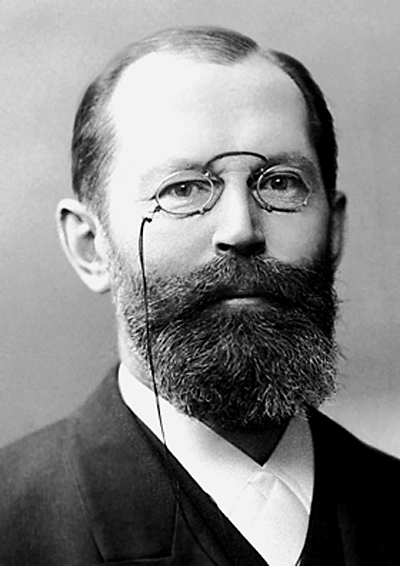
\includegraphics[width=\linewidth]{images/book3/fischer.jpg}
\end{minipage}\hfill
\begin{minipage}[t]{0.78\linewidth}
\vspace{0pt}
Emil Fischer estabeleceu, até 1891, as configurações da glicose e de seus isômeros, antes que qualquer
método físico pudesse ver uma molécula: convertendo açúcares uns nos outros e contando os estereoisômeros
obtidos. A projeção que ele inventou para escrevê-los ainda leva seu nome. Ele também preparou os
primeiros \omterm{def:b2:biomolecules:peptide}{peptídeos} sintéticos, e recebeu o Prêmio Nobel de Química de 1902. (Retrato: Atelier
Victoria, Berlim, por volta de 1895, domínio público; Wikimedia Commons.)
\end{minipage}
\end{history}

\section{Exercícios}

\begin{exercise}[$\star$]\label{exo:b2:biomolecules:1}
Desenhe a alanina como \omterm{def:b2:biomolecules:amino-acid}{zwitteríon}, depois as formas que predominam a pH 1 e a pH 12.
\end{exercise}

\begin{exercise}[$\star$]\label{exo:b2:biomolecules:2}
Calcule o \omterm{def:b2:biomolecules:amino-acid}{ponto isoelétrico} da glicina, e o da alanina ($\mathrm pK_a$ 2.35 e 9.87).
\end{exercise}

\begin{exercise}[$\star$]\label{exo:b2:biomolecules:3}
Desenhe o dipeptídeo Ala--Gly e circule sua \omterm{def:b2:biomolecules:peptide}{ligação peptídica}. Em que ele difere de Gly--Ala?
\end{exercise}

\begin{exercise}[$\star$]\label{exo:b2:biomolecules:4}
Em uma projeção de Fischer com \ce{COOH} no alto e a \omterm{def:b2:biomolecules:amino-acid}{cadeia lateral} \ce{CH2OH} embaixo, o
\ce{NH2} da serina aponta para a esquerda. Ela é D ou L? Dê seu descritor CIP.
\end{exercise}

\begin{exercise}[$\star\star$]\label{exo:b2:biomolecules:5}
Dê a carga líquida do tripeptídeo Lys--Gly--Asp a pH 1, 7 e 12.
\end{exercise}

\begin{exercise}[$\star\star$]\label{exo:b2:biomolecules:6}
Por que se usa um \omterm{def:b2:biomolecules:peptide}{agente de acoplamento} para formar uma \omterm{def:b2:biomolecules:peptide}{ligação peptídica}, em vez de um \omterm{def:b2:acyl-substitution:derivative}{cloreto de acila}
do aminoácido protegido preparado com cloreto de tionila e aquecido?
\end{exercise}

\begin{exercise}[$\star\star$]\label{exo:b2:biomolecules:7}
A D-frutose se cicliza por seu \ce{OH} de C5 sobre a cetona de C2. Dê o tamanho do anel e desenhe a
$\beta$-D-frutofuranose em \omterm{def:b2:biomolecules:anomer}{projeção de Haworth}.
\end{exercise}

\begin{exercise}[$\star\star$]\label{exo:b2:biomolecules:8}
Os \omterm{def:b2:biomolecules:anomer}{anômeros} puros da D-galactose têm rotações específicas de $+150.7$ ($\alpha$) e $+52.8$ ($\beta$) e
a mistura em equilíbrio $+80.2$ (dados do exercício). Calcule a composição no equilíbrio.
\end{exercise}

\begin{exercise}[$\star\star$]\label{exo:b2:biomolecules:9}
Explique por que a maltose reduz o licor de Fehling e a sacarose não, e por que a sacarose o reduz após
aquecimento com ácido diluído.
\end{exercise}

\begin{exercise}[$\star\star\star$]\label{exo:b2:biomolecules:10}
O índice de \omterm{def:b2:acyl-substitution:saponification}{saponificação} de uma gordura é a massa de hidróxido de potássio, em mg, que saponifica 1~g
dela. Calcule-o para a trioleína, \ce{C57H104O6}, e explique por que uma gordura de cadeias mais curtas
tem um índice mais alto.
\end{exercise}

\begin{exercise}[$\star\star\star$]\label{exo:b2:biomolecules:11}
Planeje a síntese de Gly--Ala a partir da glicina e da alanina: grupos protetores, ativação, acoplamento,
desproteção, com um par ortogonal.
\end{exercise}

\begin{exercise}[$\star\star\star$]\label{exo:b2:biomolecules:12}
Escreva a fita complementar de 5$'$-ATGCGT-3$'$, a partir de sua extremidade 5$'$, e conte as ligações
de hidrogênio que mantêm unida a fita dupla.
\end{exercise}

\section{Problema: O aspartame}

\begin{problem}[{Problema de fim de semana --- os dois aminoácidos e suas configurações, a carga do
dipeptídeo em função do pH, sua síntese e o problema $\alpha$/$\beta$, e sua hidrólise em um
refrigerante}]
\label{pb:b2:biomolecules:1}
O aspartame é o éster metílico do dipeptídeo formado pelo grupo carboxílico $\alpha$ do ácido
L-aspártico com o grupo amino da L-fenilalanina. Dados: $\mathrm pK_a$ do ácido aspártico 2.0, 3.9 e 9.9
(valores-modelo para os grupos do dipeptídeo). Massas molares (\unit{g/mol}): C 12.011, H 1.008,
N 14.007, O 15.999.
% ledger: use:aspartame, pka:asp1, pka:asp2, pka:asp3, aw:C, aw:H, aw:N, aw:O

\medskip
\noindent\textbf{Parte I --- Os dois aminoácidos.}
\begin{enumerate}
  \item Dê os três compostos liberados pela hidrólise completa do aspartame.
  \item Desenhe o ácido L-aspártico e a L-fenilalanina em projeção de Fischer.
  \item Dê o descritor CIP de cada estereocentro.
  \item Quantos estereoisômeros o aspartame tem?
  \item Desenhe o aspartame e marque a \omterm{def:b2:biomolecules:peptide}{ligação peptídica} e o éster.
  \item Por que a configuração de cada aminoácido é importante para o sabor doce?
\end{enumerate}

\medskip
\noindent\textbf{Parte II --- A carga em função do pH.}
\begin{enumerate}[resume]
  \item Liste os grupos ionizáveis do aspartame. Por que o C-terminal não é um deles?
  \item Com os valores-modelo, dê a carga líquida a pH 2.
  \item O mesmo a pH 7.
  \item O mesmo a pH 12.
  \item Estime o \omterm{def:b2:biomolecules:amino-acid}{ponto isoelétrico} neste modelo.
  \item Por que os verdadeiros valores de $\mathrm pK_a$ do dipeptídeo difeririam dos do ácido aspártico
        livre?
\end{enumerate}

\medskip
\noindent\textbf{Parte III --- Síntese.}
\begin{enumerate}[resume]
  \item Por que não se podem simplesmente aquecer juntos o ácido aspártico e o éster metílico da fenilalanina?
  \item Que grupos do ácido aspártico devem ser protegidos?
  \item O que um \omterm{def:b2:biomolecules:peptide}{agente de acoplamento} faz com o grupo carboxílico livre?
  \item O ácido aspártico tem dois grupos carboxílicos. O que se forma se o errado for acoplado?
  \item Proponha uma proteção ortogonal que deixe livre apenas o grupo carboxílico $\alpha$, e sua
        remoção.
  \item Por que o aminoácido ativado não deve ficar tempo demais em condições básicas?
  \item Escreva a sequência das etapas.
\end{enumerate}

\medskip
\noindent\textbf{Parte IV --- Hidrólise em um refrigerante.}
\begin{enumerate}[resume]
  \item Que ligações do aspartame podem ser hidrolisadas em uma bebida ácida? Qual vai primeiro?
  \item Dê os produtos da hidrólise apenas do éster.
  \item Por que um refrigerante velho tem um sabor menos doce?
  \item Calcule a massa molar do aspartame, \ce{C14H18N2O5}.
  \item Calcule a quantidade de aspartame em uma lata que contém \qty{180}{mg}.
  \item Dê a massa de metanol liberada pela hidrólise completa de \qty{180}{mg} de
        aspartame.
\end{enumerate}
\end{problem}
